\documentclass{beamer}

\usepackage{hyperref}
\usepackage{verbatim}
\usepackage{textpos}
\usepackage{multicol}
\usepackage{fancyvrb}
%\usepackage[usenames, dvipsnames]{color}
%\definecolor{Red}{rgb}{0.858, 0.188, 0.478}


\setlength{\columnseprule}{1pt}


\title{DIME Dynamic Documentation}
\author{Luiza Andrade \& Mrijan Rimal}
\institute{}
\date{\today}

\begin{document}
\begin{frame}
	\titlepage \vspace{-0.2cm}
	
\includegraphics[scale=0.25]{wbg.png} \qquad
	
\includegraphics[scale=0.25]{i2i.png} 
\end{frame}
%\frame{\titlepage \vspace{-0.2cm}

%\frame{
%	\frametitle{Overview}
%	\tableofcontents
%}

\addtobeamertemplate{frametitle}{}{%
\begin{textblock*}{100mm}(.5\textwidth,8cm)
		
\includegraphics[height=0.5cm,width=1cm]{i2i.png}
\end{textblock*}}

\frame{
\frametitle{Why is it useful for us?}
\begin{itemize}
	\item<1->Currently, a lot of us, export tables from Stata and then copy paste the tables on to Excel and then to Word or something similar. 
	\item<2->{\LaTeX} allows us to create a document once and every time a do-file is run, the tables are automatically updated in our {\LaTeX} document.
	\item<3->This saves us a lot of time in the long run even though the learning curve for {\LaTeX} is a bit complicated compared to MS Word. 
	
\end{itemize}
}
\frame{
	\frametitle{Why is it useful for us?}
	\begin{itemize}
		\item<1->Standardizes formatting across similar topics(headers, sub-headers, subsubheaders).
		\item<2->Generates Table of Contents, list of Figures, list of tables automatically.
		\item<3->Open source and standard across any version/editor of LaTeX, ShareLaTeX, etc. (not the same with Word i.e. formatting gets messed up between different version of Word).
				
	\end{itemize}
}
\frame{
	\frametitle{And....}
		\begin{itemize}
			\item<1->Documents can have comments as well. So you can write notes to yourself, future ideas which only you can read!
		\end{itemize}
}
\frame{
\frametitle{What is {\LaTeX}?}
	\begin{itemize}
		\item<1->LaTeX is a typesetting software which uses predefined formatting rules according to various settings you use(document class, page type, etc).
		\item<2->Very flexible as every setting can be defined by the user.
		\item<3->Saves a lot of time in formatting.
			\end{itemize}
}
\frame{
\frametitle{How does TeX work ?}
\begin{figure}
	\centering
	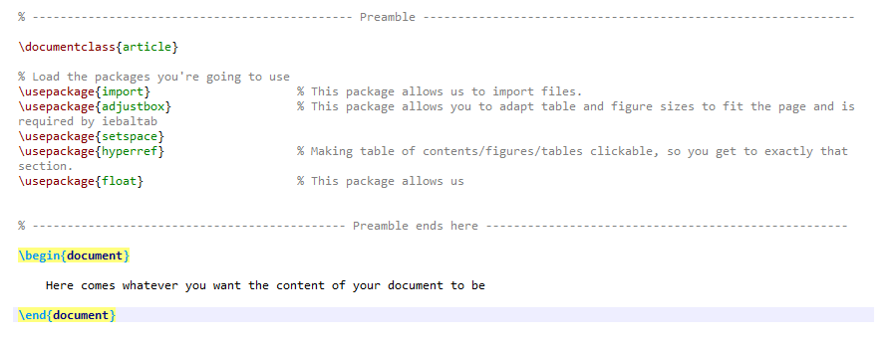
\includegraphics[scale = 0.5]{howdoestexwork.png}
\end{figure}
}
\frame{
	\frametitle{DIME LaTeX template}
	\begin{itemize}
		\item<1->Our LaTeX template allows you to display your results by just editing the path to your file.
		\item<2->Template 1 shows how to import tables.
		\item<3->Template 2 shows how to import figures.
		\item<4->Template 3 displays some more advanced options and features of {\LaTeX}.
	\end{itemize}
}
\frame{
	\frametitle{Preamble}
	\begin{figure}
		\centering
		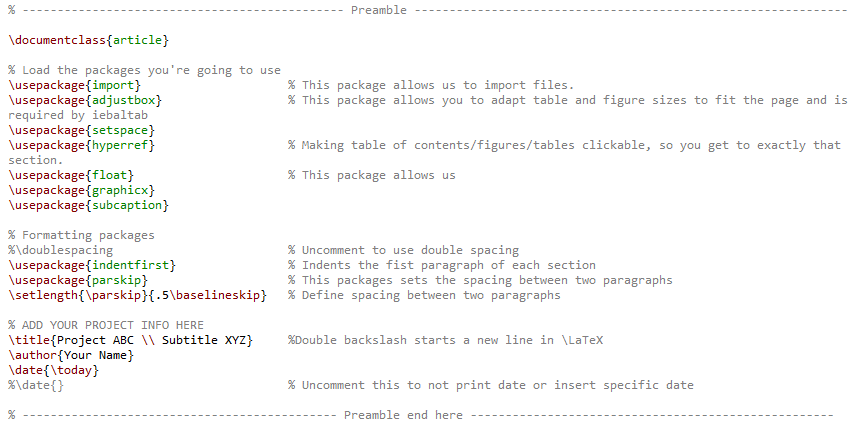
\includegraphics[scale=0.5]{preamble.png}
	\end{figure}
}

\begin{frame}[fragile]
		\frametitle{Preamble}
		\begin{itemize}
		\item<1->\begin{verbatim}
		\documentclass{article}
		\end{verbatim}
		Defines what kind of document to create. \\ \textit{Example} - article, report, book, slides, etc.
		\item<2->\begin{verbatim}
			\usepackage{package_name}
		\end{verbatim}
		You need to load the packages you want to use in the beginning of every file, otherwise it will not compile once you use the package.
		\item<3->\begin{verbatim}
		\title{document_title}
		\end{verbatim}
		The document title is defined in the preamble and later printed, as well as \textit{authors} and \textit{date}
		\end{itemize}
\end{frame}

\begin{frame}[fragile]
	\frametitle{Headers}
	\begin{figure}
		\centering
		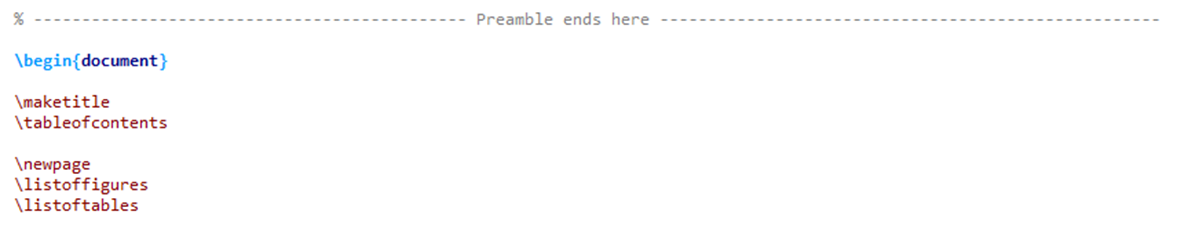
\includegraphics[width=1\linewidth]{header}
	\end{figure}
	\begin{multicols}{2}
		[]
	\begin{description}
		\tiny
		\item[maketitle] Print the document's title, authors and date in the first page.
		\item[tableofcontents] Prints a summary with all the sections and subsections.
		\item[newpage] Insert a page break.
		\item[listoffigures] Prints a list of all the figures in the document.
		\item[listoftables] Prints a list of all the tables in the document.\
		\item[Comments] Adding "\%" before text comments it out.
	\end{description}
	\columnbreak
	\begin{figure}
		\centering
		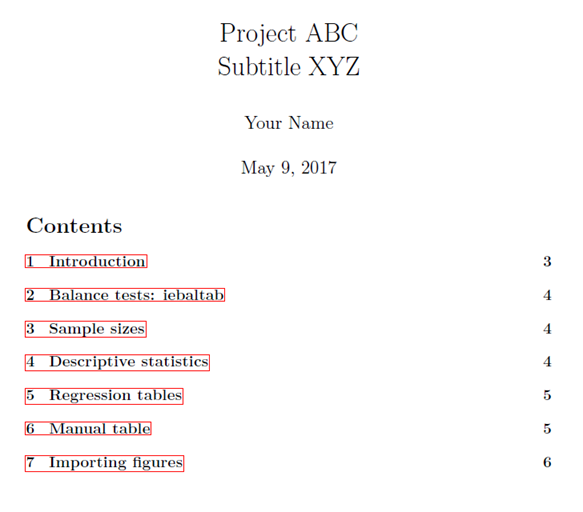
\includegraphics[width=0.8\linewidth]{preamble12}
	\end{figure}
	
	\end{multicols}
	
\end{frame}
\begin{frame}[fragile]
	\frametitle{Creating Sections}
	\begin{figure}
		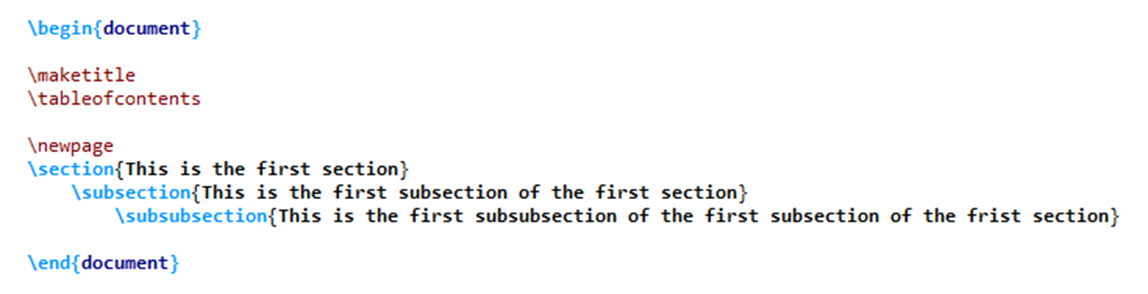
\includegraphics[width=0.7\linewidth]{sections1}
	\end{figure}
 \begin{figure}
 	\centering
 	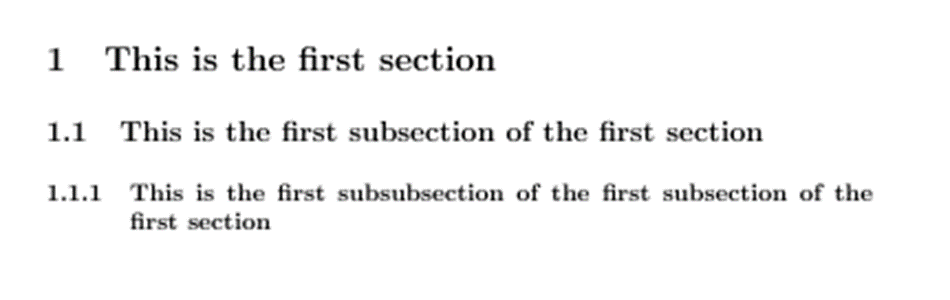
\includegraphics[width=0.7\linewidth]{sections2}
 \end{figure}
\end{frame}

\begin{frame}[fragile]
	\frametitle{Writing in your document}
	\begin{figure}
		\centering
		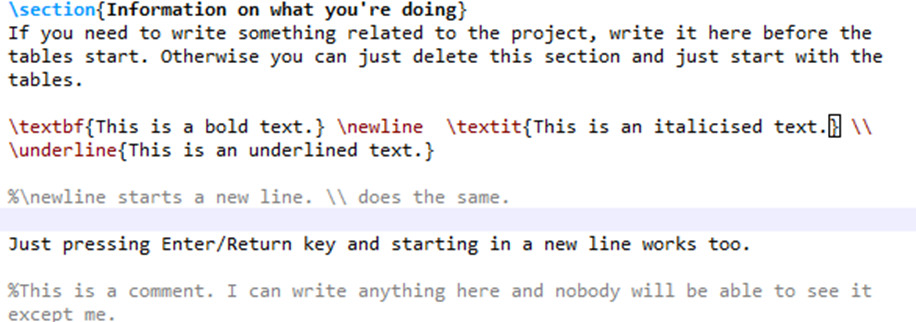
\includegraphics[width=0.7\linewidth]{writing}
	\end{figure}
\begin{figure}
	\centering
	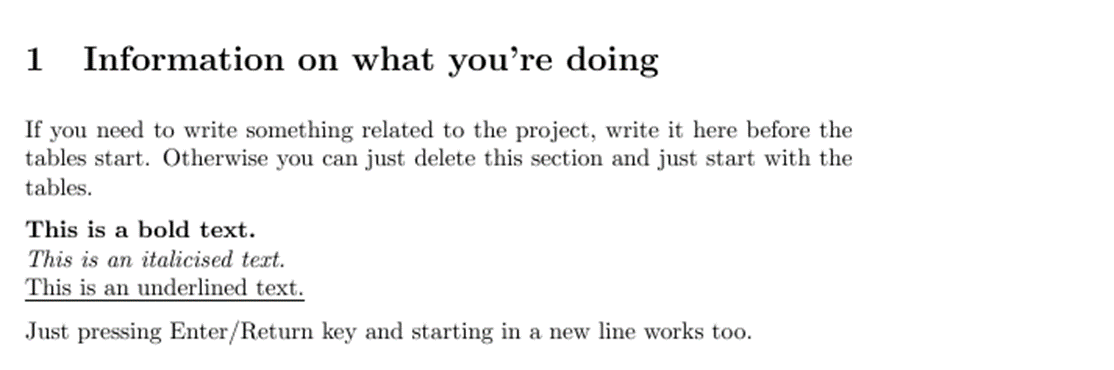
\includegraphics[width=0.7\linewidth]{writing1}
\end{figure}
\end{frame}

\begin{frame}[fragile]
	\frametitle{Importing images to your document}
	\begin{figure}
		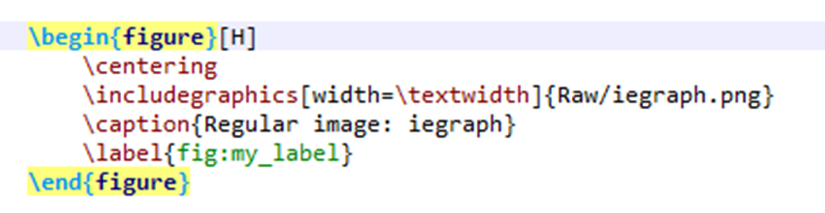
\includegraphics[width=0.7\linewidth]{import}
	\end{figure}
\begin{itemize}
	\tiny
	\item Each figure starts with \verb|\begin{figure}| and \verb|\end{figure}|
	\item \textbf{[H]} prints the figure as close as possible from where it appears in the text
	\item \verb|\centering| centers the figure (oh, really?)
	\item \verb|\includgraphics| is what actually imports your image:
	\begin{itemize}
		\tiny
		\item \verb|[width=\textwidth]| adjusts the size of the figure to the page. Alternatively, \verb|[width=0.x\textwidth]| makes it smaller.
		\item \color{red}{The path to your figure must begin from the same folder where your .tex file is!}
	\end{itemize}
	\item \verb|\caption{Name of your figure}|
	\item \verb|\label{fig:my_label}| allows you to cross-reference the figure on the text by typing \verb|\ref{fig:my_label}|
\end{itemize}
\end{frame}
\begin{frame}[fragile]
	\frametitle{Importing tables into the document}
	\begin{figure}
		\centering
		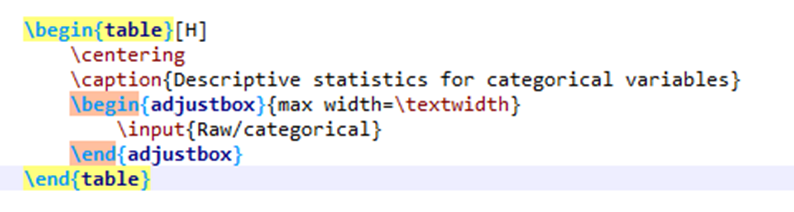
\includegraphics[width=0.7\linewidth]{import1}
	\end{figure}
	\begin{itemize}
		\tiny
		\item Each tables starts with \verb|\begin{table}| and ends with \verb|\end{table}|
		\item \verb|\begin{adjustbox}{max width = \textwidth}| adjusts the size of the table to the page. Alternatively, \verb|{max width = 0.x\textwidth}| makes it smaller.
		\item \verb|\input| is what actually imports you table
			\begin{itemize}
				\tiny
				\item \color{red}{The path to your figure must begin from the same folder where your .tex file is!}
			\end{itemize}
		\item You can also use \verb|\caption| and \verb|\label| here.  Typing \verb|\caption{}| will print “Table \#”, with no title.
		\item If \verb|\caption| comes before the table itself, the title is above it. If it comes after, the title is printed below the table.
	\end{itemize}
\end{frame}
\begin{frame}[fragile]
	\frametitle{Fragmented documents}
	\begin{figure}
		\centering
		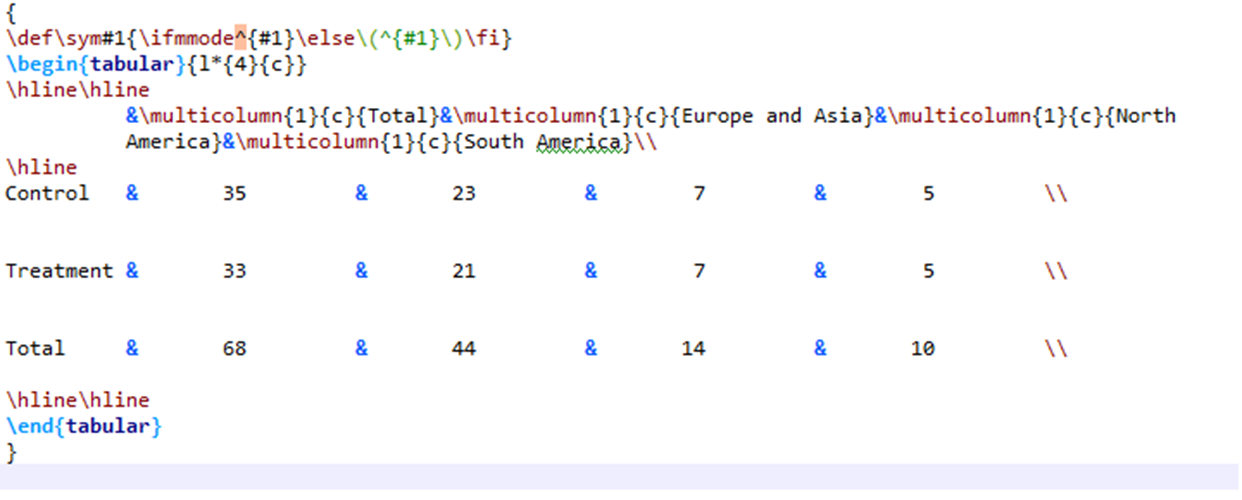
\includegraphics[width=0.7\linewidth]{fragm}
	\end{figure}
\begin{itemize}
\item The tables we export from Stata are actually fragmented documents
\item These are TeX files with no \verb|\begin{document}| or \verb|\end{document}|, so they will not compile on their own
\item We could simply copy and paste this document into our main LaTeX file, but then they would not be automatically updated
\end{itemize}
\end{frame}
	
\begin{frame}
	\frametitle{If you want to learn more…}
	\vspace*{\fill}
	\url{https://en.wikibooks.org/wiki/LaTeX}
	\vspace*{\fill}
	
\end{frame}
\end{document}
